%!TEX root = ../thesis.tex
%*******************************************************************************
%****************************** Second Chapter *********************************
%*******************************************************************************

\chapter{Related Works}
\label{chapter:related_works}

\graphicspath{{../img/related_works/}}

\par
In this chapter, we give a brief overview of the history of ML-based image
compression. Then, we focus on recent advances in lossy neural image compression
and describe and compare them against each other.

\section{Machine Learning-based Image Compression}
\par
Neural image compression goes back to at least as far as the early 1980s
(\cite{mougeot1991image}, \cite{jiang1999image}). These methods very closely
resemble in high-level structure to contemporary methods, in that they were
designed as transform coding methods. In particular, virtually all early methods
used some flavour of linear auto-encoders (LAEs, no non-linearities applied on
the hidden layer), with a single-layer encoder and
decoder (\cite{jiang1999image}). As convolutional layers had not yet been
available back then, all architectures were fully connected,
and relied on splitting up images into equal-sized blocks and feeding them
block-by-block to the LAE. Most methods optimized the MSE between the
reconstruction and the orginal image, although different learning objectives
were also explored (\cite{mougeot1991image}). Furthermore, the issue of
quantization was not formally addressed. While the pipeline was to quantize the hidden
layer activations of the LAE, no explicit treatment of the distortion introduced
by quantization was given (\cite{jiang1999image}).

\par
A notable early example of a non-neural ML-based practical compression method
is DjVu (\cite{bottou1998high}), which focused on segmenting foreground and
background in documents and using K-means clustering to for the analysis
transforming followed by entropy coding the background.

\par 
More recently, the work of \cite{denton2015deep}, \cite{gregor2015draw} focused
on discovering compressive representations using auto-encoders on low-resolution
images, using datasets such as CIFAR-10 (\cite{krizhevsky2009learning}).
\cite{toderici2015variable} proposed an RNN-based auto-encoder for compressing $32
\times 32$ thumbnails and outperformed classical methods such as JPEG and WebP
on these sizes. Their method has been later extended in \cite{toderici2017full}
for large-scale images. 

\section{Comparison of Recent Works}
\label{sec:lit_comparison}
\par
In this section we focus on compression methods that allow for the compression
of arbitrary-sized images. The most notable recent works in this area (that we
are aware of) are \cite{balle2016end}, \cite{toderici2017full}, \cite{theis2017lossy},
\cite{rippel2017real}, \cite{balle2018variational}, \cite{johnston2018cvpr} and
\cite{mentzer2018cvpr}. Of these, \cite{balle2016end}, \cite{theis2017lossy},
\cite{rippel2017real} and \cite{balle2018variational} are closest to our work and
thus we present a review of these below.

\paragraph{Note on Notation:} In this chapter, we denote the output of the
encoders by $\vec{z}$, their quantized values by $\hat{\vec{z}}$ and their
continuous relaxations by $\tilde{\vec{z}}$.

\subsection{Datasets and Input Pipelines}
\label{sec:related_works_datasets}
\par
Somewhat surprisingly, it appears that there appears to be no canonical dataset
yet for general lossy neural image compression. Such a dataset should be
comprised of a set of high-resolution, variable-sized losslessly
encoded colour images, although the CLIC Dataset (\cite{clic2018}) seems to be
an emerging one. Perhaps the reason is that generally in other domains, such as
image-based classification, cropping and rescaling images can effectively
side-step the need to deal with variable-sized images. However, when it comes
to compression, if we hope to build anything useful, side-stepping the size
issue is not an option.

\paragraph{\cite{balle2016end}} trained on 6507 images, selected from ImageNet
\cite{deng2009imagenet}. They removed images with excessive saturation and
since their method is based on dithering, they added unifrom noise to the
remaining images to imitate the noise introduced by quantization. Finally,
they downsampled and cropped images to be $256 \times 256$ pixels in size.
They only kept images whise resampling factor was 0.75 or less, in order to
avoid high frequency noise.

\paragraph{\cite{theis2017lossy}} used 434 high resolution images from \url{flickr.com}
under the creative commons license. As \texttt{flickr} store its images as
JPEGs, they downsampled all images to be below $1536 \times 1536$ in
resolution and saved them as PNGs in order to reduce the effects of the lossy
compression. Then, they extracted several $128 \times 128$ patches from each
image and trained on those.

\paragraph{\cite{rippel2017real}} took images from the Yahoo Flickr Creative Commons
100 Million dataset, with $128 \times 128$ patches randomly sampled from the
images. They do not state whether they used the whole dataset or just a
subset, neither do they describe further preprocessing steps.

\paragraph{\cite{balle2018variational}} scraped $\approx$ 1 million colour JPEG images
of dimensions at most $3000 \times 5000$. They filtered out images with
excessive saturation similarly to \cite{balle2016end}. They also
downsampled images by random factors such that the image's height and width
stayed above 640 and 1200 pixels, respectively. Finally, they use several
randomly cropped $256 \times 256$ pixel patches extracted from each image.

\paragraph{}
A clear trend is downsampling large, lossy-encoded images to get rid of the
compression artifacts as an easy way of obtaining reasonable ``approximations''
of losslessly encoded images. Another trend is that (as we see in the next
section) since all architectures are fully-convolutional, it is sufficient to
train on small image patches to train the convolution kernels to speed up
training, as well as to heavily ``increase'' the training set size.

\paragraph{Datasets for testing}
In contrast to the lack of datasets for training, all authors have used standard
datasets for testing their methods, taken from classical lossy image
compression research. These are the Kodak (\cite{kodakdataset}) and Tecnick
(\cite{asuni2014testimages}) datasets. In order for our results to be comparable
to these methods, we have also decided to test our method on the Kodak dataset.

\subsection{Architectures}
\par
This is the most diverse aspect of recent approaches, and so we will only
discuss them on a high level. We incorporated ideas from all of these papers
as well as others into our work, we discuss these in Chapter \ref{chapter:method}. All
architectures (including ours) realize a form of non-linear transform
coding. This means all architectures will have an \textit{analysis transform} or
\textit{encoder}, and a \textit{synthesis transform} or \textit{decoder} (see
Section \ref{sec:transform_coding}), both of whose parameters the methods learn
using gradient descent.
\par
All methods
achieve the ability to deal with arbitrary-sized images by only utilizing
convolutional and deconvolutional layers as their linear transformations. This
leads to the very natural consequence that the number of latent dimensions, and
thus the latent code length increases linearly in the number of pixels of the
input image. They all utilise downsampling after some convolutions.
Every work that gives details
on how they perform downsampling do it by using a stride larger than 1 on the
convolutions, and it is reasonable to assume that the rest do it likewise.
Padding and convolution mode is generally not discussed except in
\cite{theis2017lossy}, but we believe all other methods use one of the two ways
they present, namely zero-padded or mirror-padded convolutions in \texttt{same}
mode. The further details of each individual work is detailed below.

\paragraph{\cite{balle2016end}} They build a relatively shallow autoencoder (5
layers) (Shown in the left half of Figure \ref{fig:balle_ladder_arch}).
They propose their own activation function, custom tailored for image
compression. These non-linearities are a form of adaptive local gain control
for the images, called Generalized Divisive Normalization (GDN). At the $k$th layer for
channel $i$ at position $(m, n)$, for input $w_i^{(k)}(m, n)$, the GDN
transform is defined as
\begin{equation}
  \label{eq:gdn_def}
  u_i^{(k + 1)}(m, n) = \frac{w_i^{(k)}(m, n)}{
    \left( \beta_{k, i} + \sum_j \gamma_{k, i, j}
      \left( w_{j}^{(k)}(m, n)\right)^2 \right)}.
\end{equation}
Its approximate inverse, IGDN for input $\hat{u}_i^{(k)}(m, n)$ is defined as
\begin{equation}
  \label{eq:igdn_def}
  \hat{w}_i^{(k)}(m, n) = \hat{u}_i^{(k)}(m, n) \cdot \left(
    \hat{\beta}_{k, i} + \sum_{j} \hat{\gamma}_{k, i, j} \left(
      \hat{u}_j^{(k)}(m, n)\right)^2 \right)^{\frac{1}{2}}.
\end{equation}
Here, the set $\beta_{k, i}, \gamma_{i, j, k}, \hat{\beta}_{k, i},
\hat{\gamma}_{i, j, k}$ are learned during training and fixed at test time.

\paragraph{\cite{theis2017lossy}} They define a Compressive Autoencoder (CAE) as a regular
autoencoder with the quantization step between the encoding and decoding step.
(In this sense, the architectures of \cite{balle2016end} and
\cite{balle2018variational} are also CAEs.) They mirror pad the input first
and then they follow it up by a deep, fully convolutional, residual
architecture \cite{he2016deep}. They use valid convolutions and downsample by
using a stride of 2. Between convolutions they use leaky ReLUs as
nonlinearities, which are defined as 
\[
  f_\alpha(x) = \max\{x, \alpha x\}, \quad \alpha \in [0, 1].
\]
The decoder mirrors the encoder. When upsampling is required, they use what
they term \textit{subpixel} convolutions, where they perform a regular
convolution operation with an increased number of filters, and then reshape
the resulting tensor into one with larger spatial extent but fewer channels.
Their architecture can be seen in Figure \ref{fig:comp_auto_arch}.
\begin{figure}
  \centering 
  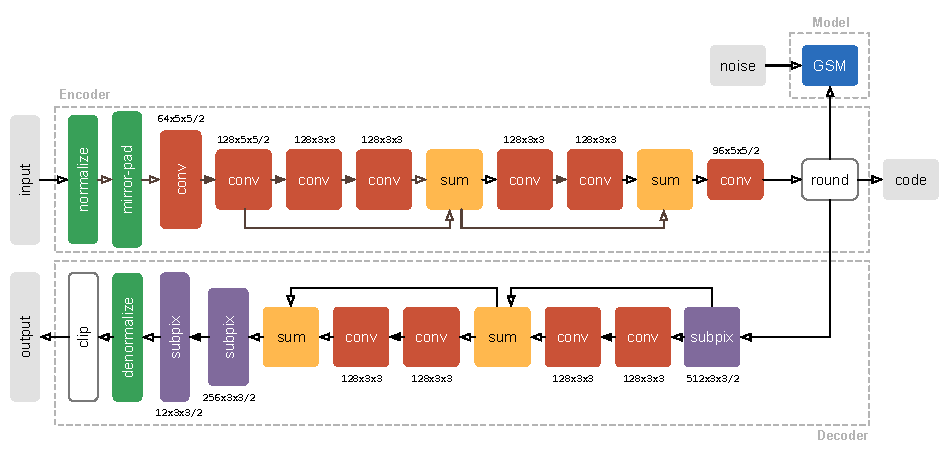
\includegraphics[width=\textwidth]{compressive_autoencoders_architecture.pdf}
  \caption{Compressive Auto-Encoder architecture used by \cite{theis2017lossy}.
    Note that for visual clarity only 2 residual blocks are displayed,
    in their experiments they used 3. They use a 6-component Gaussian Scale
    Mixture model (GSM) to model the quantization noise during the training of
    the architecture. The normalization layer performs batch normalization
    separately for each channel, denormalization is the analogous inverse
    operation. (Image taken from their \cite{theis2017lossy}.)}
  \label{fig:comp_auto_arch}
\end{figure}

\paragraph{\cite{rippel2017real}} They use a reasonably shallow architecture as well,
but also add in an additional residual connections from every layer to the last,
summing at the end. They call this
\textit{pyramidal decomposition} and \textit{interscale alignment}, with the
rationale behind it being that the residual connections extract features at
different scales, and so the latent representations can take advantage of this.
Their encoder architecture is shown in Figure \ref{fig:rippel_arch}.
\begin{figure}
  \centering 
  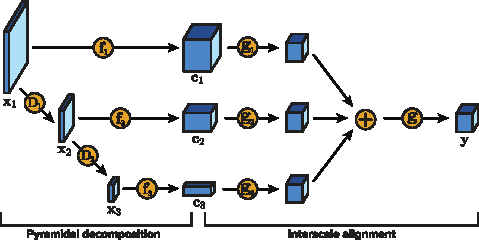
\includegraphics[width=0.7\textwidth]{rippel_architecture.pdf}
  \caption{Encoder architecture used by \cite{rippel2017real}. All circular blocks
    denote convolutions. (Image taken from \cite{rippel2017real}.)}
  \label{fig:rippel_arch}
\end{figure}
\paragraph{\cite{balle2018variational}} They extend the architecture presented in
\cite{balle2016end}, see Figure \ref{fig:balle_ladder_arch}.
In particular, the encoder and decoder remain the same,
and they add an additional stochastic layer on top of the architecture,
resembling a probabilistic ladder network (PLN) (\cite{sonderby2016train}).
The layers leading to the second level are more standard. They are still fully
convlutional with downsampling after convolutions, however, instead of GDN
they use ReLUs.
\par

\begin{figure}
  \centering 
  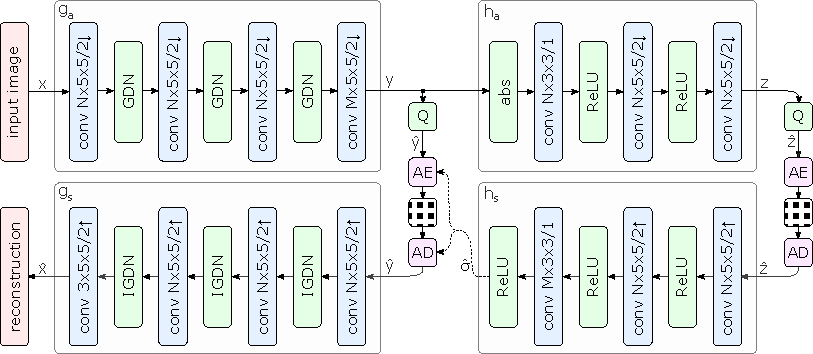
\includegraphics[width=\textwidth]{balle_ladder_architecture.pdf}
  \caption{Analysis and synthesis transforms $g_a$ and $g_s$ along with first
    level quantizer $Q(\vec{y})$ used in \cite{balle2016end}. This architecutre
    was then extended by \cite{balle2018variational} with second level analysis
    and synthesis transforms $h_a$ and $h_s$, along with second level quantizer
    $Q(\vec{z})$. This full architecture is also the basis of our model. A
    slightly strange design choice on their part is since they will wish to
    force the second stage activations to be positive (it will be predicting
    a scale parameter), instead of using an exponential or softplus
    ($\log (1 + \exp\{x\})$) activation at the end, they take the absolute value
    of the input to the first layer, and rely on the ReLUs never giving negative
    values. We are not sure if this was meant to be a computational saving, as
    taking absolute values is certainly cheaper then either of the
    aforementioned standard ways of forcing positive values, or it if it gave
    better results.
    (Image taken from \cite{balle2018variational})}
  \label{fig:balle_ladder_arch}
\end{figure}

\subsection{Addressing Non-Differentiability}
\label{sec:comp_quant}
\par
As all methods surveyed here are trained using gradient-based methods, a crucial
question that needs to be answered is how they dealt with the issue of
quantization. This is because end-to-end optimizing the transform coding
pipeline involves back-propagating gradients through the quantization step, which
yields 0 derivatives almost everywhere, stopping the learning signal.
In fact, there are two issues that need to be addressed and that we examine
below: first, the quantization operation itself, and second,
the rate estimator $H[P(\vec{z})]$ (except for \cite{rippel2017real} as they do
not use it). As we have
seen in Section \ref{sec:compression_without_quantization}, not only is there
inherent error in whatever approximation is used to circumvent the
non-differentiability of quantization, the use of quantization itself already
fundamentally limits how
effective these methods can be. A graphical representation of various continuous
relaxations / approxiamtions of quantization error can be seen in Figure
\ref{fig:quantization_models}. 
\begin{figure}
  \centering 
  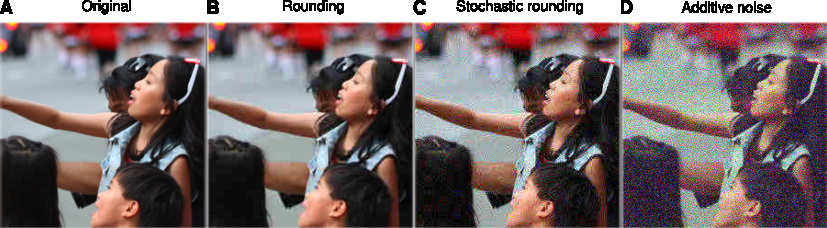
\includegraphics[width=\textwidth]{compressive_autoencoders_quant_comparison.pdf}
  \caption{Comparison of quantization error and its relaxations. \textbf{A)}
    Original image. \textbf{B)} Artifacts that result from using rounding as the
    quantizer. \textbf{C)} Stochastic rounding used by \cite{toderici2017full}.
    \textbf{D)} Uniform additive noise used by \cite{balle2016end} and
    \cite{balle2018variational}. (Image taken from \cite{theis2017lossy}.)}
  \label{fig:quantization_models}
 \end{figure}

\subsubsection{Quantization}
\par
All methods use some form of rounding $\vec{z}$ as
\begin{equation}
\label{eq:quantization_step}
  \hat{z}_i = \frac{1}{2^B}\left[2^B \times z_i\right], 
\end{equation}
for some $B$ (usually $B = 0$). Below we see what continuous relaxations are used
during training time.
 
\paragraph{\cite{balle2016end} and \cite{balle2018variational}}
They model quantization
error as dither, i.e. they replace their quantized latents
$\hat{z}_i$ by additive unifrom noise
\[
  \tilde{z}_i = z_i + \delta z_i, \quad \delta z_i \sim \Unif{0, 1}. 
\]

\paragraph{\cite{theis2017lossy}} They replace the derivative of the rounding
operation in the backpropagation chain by the constant function 1:
\[
  \frac{d}{d y} [y] = 1.
\]
This is a smooth approximation of rounding and they report that empirically it
gave good results. However, as quantization itself creates an important
bottleneck in the flow of information, it is key that only the derivative is
replaced during the backward pass and not the operation itself during the
forward pass.

\paragraph{\cite{rippel2017real}} use $B = 6$ in Eq \ref{eq:quantization_step},
however, they do not reveal their relaxation of the quantization step during
the learning phase. They cite \cite{balle2016end} and \cite{toderici2017full}
though, so our best guess is that they most likely picked a method proposed in
either one of those.

\subsubsection{Rate Estimation}
\par
As all methods but \cite{rippel2017real} under review aim to optimize
the rate-distrotion trade-off
directly, they also need to estimate the rate $H[\hat{\vec{z}}] = -\Exp{\log
  P(\hat{\vec{z}})}{P(\hat{\vec{z}})}$. Hence to model the rate during training,
they also require a distribution over the $\tilde{z}_i$s.

\paragraph{\cite{balle2016end}}
  They assume that the latents are independent, and hence they
  can model the the joint as a fully factorized distribution. They use linear
  splines to do this, whose parameters $\psi^{(i)}$ they update separately every
  $10^6$ iterations using SGD to maximize its log-likelihood on the latents,
  independently from the optimization of the rest of the model parameters.
  Then, they use this prior to replace the entropy term as
  \[
   H[\tilde{\vec{z}}] = \Exp{-\sum_i \log_2 p(z_i + \delta z_i \mid \psi^{(i)})}{}.
  \]

\paragraph{\cite{theis2017lossy}} They note that
  \[
    P(\vec{z}) = \int_{\left[-\frac{1}{2}, \frac{1}{2}\right)^M} q(\vec{z} + \vec{u}) \d \vec{u}
  \]
  for some appropriate density $q$,
  where the integral is taken over the centered $M$ dimensional hypercube.
  Then, they replace the the rate estimator with an upper bound using Jensen's
  inequality:
  \[
    -\log_2P(\vec{z}) = -\log_2\int_{\left[-\frac{1}{2}, \frac{1}{2}\right)^M} q(\vec{z} +
    \vec{u}) \d \vec{u} \leq -\int_{\left[-\frac{1}{2}, \frac{1}{2}\right)^M} \log_2q(\vec{z} +
    \vec{u}) \d \vec{u}.
  \]
  This upper bound is now differentiable. They pick Gaussian Scale Mixtures for
  $q$, with $s = 6$ components, with the mixing proportions fixed across spatial
  dimensions, which gives the negative log likelihood
  \[
    -\log_2 q(\vec{z} + \vec{u}) =
    \sum_{i, j, k} \log_2 \sum_s \pi_{k, s} \Norm{z_{k,i,j} + u_{k, i, j} \mid
    0, \sigma_{k, s}^2},
  \]
  where $i,j$ iterate through the spatial dimensions and $k$ indexes the
  filters. The integration of this in the architecture can be seen in Figure
  \ref{fig:comp_auto_arch}.  This allows them to replace the rate estimator with
  \[
    H[\tilde{\vec{z}}] = -\Exp{\log_2 q(\vec{z} + \vec{u})}{}.
  \]

  \paragraph{\cite{balle2018variational}} They us a non-parametric,
  fully factorized prior for the second stage:
  \[
    p(\tilde{\vec{z}}^{(2)} \mid \psi) =
    \prod_i \left(  p\left(\tilde{z}^{(2)}_i \mid \psi_i\right) *
      \Unif{-\frac{1}{2}, -\frac{1}{2}\right)}.
  \]
  Then, they model the first stage as dithered zero-mean Gaussians with variable
  scale depending on the second stage, thereby relaxing the initial independence
  assumption on the latent space to a more general \textit{conditional
    indepenence} assumption \cite{bishop1998latent}:
  \[
    p(\tilde{\vec{z}}^{(1)} \mid \tilde{\vec{z}}^{(2)}) = 
    \prod_i \left(  \Norm{\tilde{z}^{(1)}_i \mid 0, \tilde{\sigma}^2_i\right)*
      \Unif{-\frac{1}{2}, -\frac{1}{2}}}.
  \]
  They then replace the rate estimator similarly to \cite{balle2016end}.

\subsection{Coding}
\par
Another important part of the examined methods is the entropy coding. In particular, an
interesting caveat of entropy codes is that they tend to perform slightly worse
than the predicted rate, due to neglected constant factors in the algorithm
\cite{rissanen1981universal}. Hence, it is always more informative to present
results where the actual coding has been performed and not just the theoretical
rate reported. All examined works have implemented their own coding algorithms,
and we briefly review them here. 

\paragraph{\cite{balle2016end}} Use a context adaptive binary arithmetic coding (CABAC).
  They code dimensions in raster-scan order, which means they do not fully leverage the
  spatial dependencies between adjacent latent dimensions.
  As the authors note, this means that CABAC does not yield much improvement
  over non-adaptive artihmetic coding. 

\paragraph{\cite{theis2017lossy}} used their estimated probabilities $q(\vec{z})$ and
  used an off-the-shelf publicly available range coder to compress their latents.

\paragraph{\cite{rippel2017real}} treat each bit of their $B$-bit precision quantized
  representations individually, because they want to utilize the sparsity of
  more significant bits. They train a separate binary classifier to predict
  probabilities for each individual bit based on a set of features (they call
  it a \textit{context}) to use in an adaptive arithmetic coder. They further
  add a regularizing term during training based on the codelength of a batch to
  match a length target. This is to encourage sparsity for high-resolution, but
  low entropy images and a longer codelength for low resolution but high entropy
  images.

\paragraph{\cite{balle2018variational}} use a non-adaptive arithmetic coder as their
  entropy code. As they have two stochastic levels, with the
  first depending on the second, they have to code them sequentially. For the
  second level, they get their frequency estimates for $\hat{\vec{z}}^{(2)}$
  from the non-parametric prior:
  \[
    p(\hat{z}^{(2)}_i) =
    \int_{\hat{z}^{(2)}_i-\frac{1}{2}}^{\hat{z}^{(2)}_i+\frac{1}{2}}p(\tilde{z}_i \mid \psi_i) \d \tilde{z}_i.
  \]
  Then, on the first level, their probaibilities are given by:
  \[
    p(\hat{z}^{(1)} \mid \tilde{z}^{(2)}) = p(\hat{z}^{(1)} \mid
    \tilde{\sigma}^2_i) = 
    \int_{\hat{z}^{(1)}_i-\frac{1}{2}}^{\hat{z}^{(1)}_i + \frac{1}{2}}\Norm{\tilde{z}_i \mid 0, \tilde{\sigma}^2_i} \d \tilde{z}_i.
  \]

\subsection{Training}
\par
\cite{balle2016end}, \cite{theis2017lossy} and \cite{balle2018variational}
optimize the rate-distrotion trade-off directly,
\[
  L(\Data) = H[\hat{\vec{z}}] + \beta \Exp{d(\vec{x}, \hat{\vec{x}})}{},
\]
where the expectation is taken over training batches. This turns out to be
equivalent to maximizing the ELBO for a certain VAE, whereas \cite{rippel2017real} use a
more complex loss function, see below for details. All methods train their model
using Adam \cite{kingma2014adam}, but most do not state the number of
training epoch.

\paragraph{\cite{balle2016end}} Since they use MSE as the distance metric,
they note that their
architecture could be considered as a (somewhat
unconventional), VAE with Gaussian likelihood
\[
  p(\vec{x} \mid \tilde{\vec{z}}, \beta) =
  \Norm{\vec{x} \mid \hat{\vec{x}}, (2\beta)^{-1}\vec{1}},
\]
mean-field prior
\[
  p(\tilde{\vec{z}} \mid \psi^{1}, \hdots, \psi^{N}) =
  \prod_i p(\tilde{z}_i \mid \psi^{(i)})
\]
and mean-field posterior
\[
  q(\tilde{\vec{z}} \mid \vec{x}) =
  \prod_i \Unif{\tilde{z}_i \mid z_i, 1},
\]
where $\Unif{\tilde{z}_i \mid z_i, 1},$ is the uniform distribution centered
on $z_i$ of width 1. They used learning rate decay during training.

\paragraph{\cite{theis2017lossy}}
  They performed the training incrementally, in the sense that they masked most
  latents at the start, such that their contribution to the loss was 0. Then, as
  the training performance saturated, they unmasked them incrementally. They
  also used learning rate decay during training.

\paragraph{\cite{rippel2017real}} They use a complex loss function, with an MS-SSIM
distrotion cost, a code length regularization term (not equivalent to the rate
term) as well as an adversarial loss term. In their adversarial setup they feed
ground truth, reconstruction pairs to the discriminator, where they shuffle the
images in the pair with probability $\frac12$ and their discriminator was
trained to predict which image was the reconstruction. Their setup can be seen
in Figure \ref{fig:rippel_pipeline}. To stabilize the
adversarial training procedure, they also introduce an adaptive learning signal
scheduler, preventing any of the signals from dominating the total.
\begin{figure}
  \centering 
  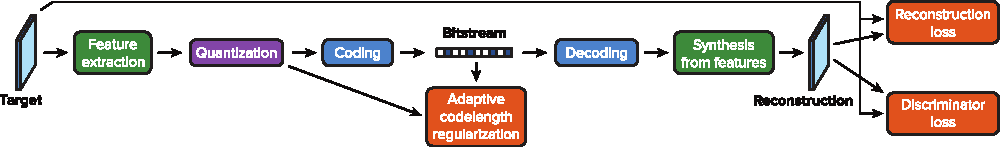
\includegraphics[width=\textwidth]{rippel_pipeline.pdf}
  \caption{Compression pipeline used by \cite{rippel2017real}. The red boxes
    show the terms used in their loss function. (Image taken from \cite{rippel2017real}.)}
  \label{fig:rippel_pipeline}
\end{figure}

\paragraph{\cite{balle2018variational}} In the same vein as they laid out their
  VAE-based training objective in \cite{balle2016end}, the data log-likelihood
  term stays, but now the regularizing term is the KL divergence between the
  joint posterior $q(\tilde{\vec{z}}^{(1)}, \tilde{\vec{z}}^{(2)} \mid \vec{x})$
  and the joint prior 
  $q(\tilde{\vec{z}}^{(1)}, \tilde{\vec{z}}^{(2)})$. Here, as due to the
  dithering assumption, the joint posterior works out to be
  \[
    q\left(\tilde{\vec{z}}^{(1)}, \tilde{\vec{z}}^{(2)} \mid \vec{x}\right) =
    \prod_i \Unif{\tilde{z}^{(1)}_i \mid \hat{z}^{(1)}, 1} \cdot
    \prod_i \Unif{\tilde{z}^{(2)}_i \mid \hat{z}^{(2)}, 1}.
  \]
  \par
  Then, taking the KL between these, the full traning objective works out to be
  \begin{equation}
    \label{eq:balle_var_train_objective}
    L = \Exp{ -\sum_i \log_2 p(\tilde{z}^{(2)}_i \mid \psi^{(i)}) 
      -\sum_i \log_2 p(\tilde{z}^{(1)}_i \mid \tilde{\sigma}^2_i) +
      \beta d(\vec{x}, \hat{\vec{x}})}{}.
  \end{equation}
  Eq \ref{eq:balle_var_train_objective} is important from our prespective, as
  it will be
  directly translated to our learning objective.
  \par
  They train 32 models, half using the architecture from \cite{balle2016end} and
  half using the current one, half optimized for MSE and half of MS-SSIM, with 8
  different $\beta$s. They report that neither batch normalization nor learning
  rate decay gave better results, which they attribute to GDN.

\subsection{Evaluation}
\par
As mentioned at the end of Section \ref{sec:related_works_datasets}, all
methods were tested on the Kodak dataset (\cite{kodakdataset}). All authors
report the (interpolated) rate-distrotion curves achieved by their models. All
methods report the curves using PSNR (\cite{psnr}) as the distrotion metric as
well as MS-SSIM (\cite{msssim}), except for \cite{rippel2017real}, who only
report MS-SSIM. Based on these reported curves, the current state-of-the-art in
neural compression is set by \cite{balle2018variational}. 
\par
An important issue raised in \cite{balle2016end} and \cite{balle2018variational}
is how aggregate results over should be reported, or whether reporting such
figures is meaninful in the first place. This is because since models were
trained on different datasets, with different model design philosophies, there
might be significant fluctuation in the comparative model performance between
individual images. Furthermore, averaging results achieved by classical methods
that were not directly optimized for the rate-distrotion trade-off (virtually
all of them) might lead to inconsistent results even on the same image, depending on what settings were used to achieve
a given bitrate. Hence, they argue that the efficiency of the methods should
be examined on individual images instead. This is also the philosophy we follow,
and hence we will be reporting model performances on individual images.